\documentclass[rgb,dvipsnames]{beamer}

\usepackage[english]{babel}
\usepackage{xcolor}
\usepackage{listings}
\usepackage{adjustbox}
\newcommand{\LO}{$\mathcal{L}_0$}
\usepackage{amsmath}
\usepackage{multirow}

\usepackage[linewidth=1pt]{mdframed}

% Graphics
\usepackage{graphicx}

% Font
\usepackage{paratype}
\setbeamerfont{frametitle}{family=\bf}

% Beamer theme settings
\usecolortheme{seagull}
\setbeamertemplate{itemize item}{\raisebox{0.8mm}{\rule{1.2mm}{1.2mm}}}
\usenavigationsymbolstemplate{} % no navigation buttons

\lstdefinelanguage{Futhark}
{keywords={fun,if,then,else,loop,do,map,reduce,filter,scan,redomap,transpose,reshape,iota,replicate,let,in,for,while,with,f32,int,i8,u8,zip,streamRed,zipWith,unsafe,module,type,val,i32},%
  sensitive=true,%
  comment=[l]{--},%
  string=[b]",%
  moredelim=**[is][\color{red}]{@}{@},
  moredelim=**[is][\color{blue}]{¤}{¤},
}

\lstset{
  language=Futhark,
  basicstyle=\footnotesize
}

\usepackage{epic}
\usepackage{amsmath}
\usepackage{amssymb}
\usepackage{amsthm}

\newcommand{\basetop}[1]{\vtop{\vskip-1ex\hbox{#1}}}
\newcommand{\source}[1]{\let\thefootnote\relax\footnotetext{\scriptsize\textcolor{kugray1}{Source: #1}}}

% for coloured code citation in text:
\usepackage{fancyvrb}

%%%%%%%%%%%%%%%%%%%%%%%%%%%%%%%%%
%%%%%    code sections   %%%%%%%%
%%%%%%%%%%%%%%%%%%%%%%%%%%%%%%%%%

% code highlighting commands in own block
\DefineVerbatimEnvironment{code}{BVerbatim}{}
\DefineVerbatimEnvironment{icode}{Verbatim}{fontsize=\scriptsize}
\DefineVerbatimEnvironment{tinycode}{Verbatim}{fontsize=\tiny}


% Fancy code with color commands:
\DefineVerbatimEnvironment{colorcode}%
        {Verbatim}{fontsize=\scriptsize,commandchars=\\\{\}}

%%%%%%%%%%%%%%%%%%%%%%%%%%%%%%%%%%
%%%%%    some coloring    %%%%%%%%

%% use "DIKU green" from our color theme for \emph
%\renewcommand{\emph}[1]{\textcolor{structure}{#1}}
%% use some not-too-bright red for an \emp command
%\definecolor{DikuRed}{RGB}{130,50,32}
%\newcommand{\emp}[1]{\textcolor{DikuRed}{ #1}}
%\definecolor{CosGreen}{RGB}{10,100,70}
%\newcommand{\emphh}[1]{\textcolor{CosGreen}{ #1}}


\definecolor{Red}{RGB}{220,50,10}
\definecolor{Blue}{RGB}{0,51,102}
\definecolor{Yellow}{RGB}{102,51,0}
\definecolor{Orange}{RGB}{178,36,36}
\definecolor{Grey}{RGB}{180,180,180}
\definecolor{Green}{RGB}{20,120,20}
\definecolor{Purple}{RGB}{160,50,100}
\newcommand{\red}[1]{\textcolor{Red}{{#1}}}
\newcommand{\blue}[1]{\textcolor{Blue}{{#1}}}
\newcommand{\yellow}[1]{\textcolor{Yellow}{{#1}}}
\newcommand{\orange}[1]{\textcolor{Orange}{{#1}}}
\newcommand{\grey}[1]{\textcolor{Grey}{{#1}}}
\newcommand{\green}[1]{\textcolor{Green}{{#1}}}
\newcommand{\purple}[1]{\textcolor{Purple}{{#1}}}




% use "DIKU green" from our color theme for \emph
\renewcommand{\emph}[1]{\textcolor{structure}{#1}}
% use some not-too-bright red for an \emp command
\definecolor{DikuRed}{RGB}{130,50,32}
\newcommand{\emp}[1]{\textcolor{DikuRed}{ #1}}
\definecolor{CosGreen}{RGB}{10,100,70}
\newcommand{\emphh}[1]{\textcolor{CosGreen}{ #1}}
\definecolor{CosBlue}{RGB}{55,111,122}
\newcommand{\emphb}[1]{\textcolor{CosBlue}{ #1}}
\definecolor{CosRed}{RGB}{253,1,1}
\newcommand{\empr}[1]{\textcolor{CosRed}{ #1}}

\newcommand{\mymath}[1]{$ #1 $}
\newcommand{\myindx}[1]{_{#1}}
\newcommand{\myindu}[1]{^{#1}}

\newtheorem{mydef}{Definition}
\newtheorem{mytheo}{Theorem}
\newtheorem{mylemma}{Lemma}

%%%%%%%%%%%%%%%%%%%%


\title[Intro]{Short Intro to Futhark}

\author[C.~Oancea]{Cosmin E. Oancea\\{\tt cosmin.oancea@diku.dk}}

\institute{Hiperfit, DIKU\\
  University of Copenhagen\\ \includegraphics[width=1cm]{img/hiperfitlogo.png}    \includegraphics[width=1cm]{img/diku-logo2.png}}

\date{may 2017}




\begin{document}

%\titleslide

%\begin{frame}[fragile,t]
%  \frametitle{Map, Reduce, and Scan Types and Semantics}
%
%\begin{itemize}
%    \item \emp{\tt map~::~($\alpha\rightarrow\beta$)~$\rightarrow$~[$\alpha$]$~\rightarrow$~[$\beta$]}\\
%    \emph{\tt map f [x$_1,\ldots, $x$_n$] = [f(x$_1$),$\ldots$, f(x$_n$)]},\\  
%        i.e., \emp{\tt{}x$_i$~::~$\alpha, \forall i$}, and 
%        \emp{\tt f~::~$\alpha\rightarrow\beta$}.\medskip
%
%    \item \emp{{\tt reduce~::~($\alpha$~$\rightarrow$~$\alpha$~$\rightarrow$~$\alpha$)~$\rightarrow$~$\alpha$~$\rightarrow$~[$\alpha$]~$\rightarrow$~$\alpha$}}\\
%        \emph{\tt reduce $\odot$~e~[x$_1$,x$_2$,..,x$_n$]~=~e$\odot$x$_1\odot$x$_2\odot\ldots\odot$x$_n$},\\
%        i.e., \emp{{\tt{}e::$\alpha$, x$_i$~::~$\alpha, \forall i$}}, and 
%        \emp{\tt $\odot$~::~$\alpha\rightarrow\alpha\rightarrow\alpha$}.\medskip
%
%    \item \emp{{\tt scan$^{exc}$~::~($\alpha$~$\rightarrow$~$\alpha$~$\rightarrow$~$\alpha$)~$\rightarrow$~$\alpha$~$\rightarrow$~[$\alpha$]~$\rightarrow$~[$\alpha$]}}\\
%        \emph{\tt scan$^{exc}~\odot$~e~[x$_1$,$\ldots$,x$_n$]~=~[e,e$\odot$x$_1$,$\ldots$,e$\odot$x$_1\odot\ldots$x$_{n-1}$]}\\
%        i.e., \emp{{\tt{}e::$\alpha$, x$_i$~::~$\alpha, \forall i$}}, and 
%        \emp{\tt $\odot$~::~$\alpha\rightarrow\alpha\rightarrow\alpha$}.\medskip
%
%    \item \emp{{\tt scan$^{inc}$~::~($\alpha$~$\rightarrow$~$\alpha$~$\rightarrow$~$\alpha$)~$\rightarrow$~$\alpha$~$\rightarrow$~[$\alpha$]~$\rightarrow$~[$\alpha$]}}\\
%        \emph{\tt scan$^{inc}~\odot$~e~[x$_1$,$\ldots$,x$_n$]~=~[e$\odot$x$_1$,$\ldots$,e$\odot$x$_1\odot\ldots$x$_{n}$]}\\
%        i.e., \emp{{\tt{}e::$\alpha$, x$_i$~::~$\alpha, \forall i$}}, and 
%        \emp{\tt $\odot$~::~$\alpha\rightarrow\alpha\rightarrow\alpha$}.
%
%\end{itemize}
%
%\end{frame}

\begin{frame}[fragile,t]
   \frametitle{Motivation: Higher-Level Parallel Programming}

\begin{description}
    \item[\emphh{Moore's Low'60:}] computer power doubles every 19-24 months.\medskip
    \item[\emphh{Since mid-2000:}] all current and future architectures adopt some form of massive parallelism,
            but massively parallel hardware is capricious and difficult to program.\medskip 
            %(as the only way to keep Moore's Low alive)
    \item[\emphh{Main Challenge:}] productivity tools for quickly writing programs that run fast (enough).\medskip
\end{description}
\bigskip

\emph{How do we tackle this?}
\begin{itemize}
    \item[1] ``think parallel'' language abstraction\\
            (because loops are unsuitable for expressing parallelism).\medskip
    \item[2] interoperability mechanisms with programming-productivity environments, e.g., Python, C, Java, etc.
\end{itemize}

\end{frame}

\begin{frame}[fragile,t]
   \frametitle{Think Parallel: Basic Blocks of Parallel Programming}

Notation: 
\begin{itemize}
    \item $[a_1,\ldots,a_n]$ denotes an array literal,
    \item $(\alpha_1,\ldots,\alpha_n)$ denotes a tuple (record),
    \item $[n]\alpha$ denotes the type of an array with $n$ elements of type $\alpha$.
\end{itemize}
\bigskip

\emph{\bf Parallel programs can be built by a nested composition of bulk-parallel array operators.} 

\bigskip


\emphh{iota : $(n:int) \ \rightarrow \ [n]int$}\\
\emphh{iota}(n) $\equiv$ $[0, 1, \ldots, n-1]$\\\bigskip

\emphh{replicate} : $(n:int, \ \alpha) \rightarrow [n]\alpha$\\
\emphh{replicate}(n, a) $\equiv$ $[a, \ldots, a]$\\\bigskip

\emphh{zip} : $([n]\alpha, \ [n]\beta) \ \rightarrow [n](\alpha,\beta)$\\
\emphh{zip} ($[a_1, \ldots, a_n], \ [b_1, \ldots, b_n]$) $\equiv$ $[(a_1,b_1), \ldots, (a_n,b_n)]$\\\bigskip

\emphh{unzip} $\equiv$ zip$^{-1}$


%\bigskip
%\bigskip

%\emp{Map Fusion:} (higher-order transformation)
%
%\begin{tabular}{rccc}
%a = & \{ $a_1$, $a_2$, .., $a_n$ \} & & a = \{ $a_1$, $a_2$, .., $a_n$ \} \\  
%\emp{x =} & \emp{map~f~a} & & \\
%%  & $\downarrow$ & & \\
%%//x = &  \{ \emph{f($a_1$)}, \emph{f($a_2$)}, .., \emph{f($a_n$)} \} & & \\
%\emph{y} = & \emp{map~g~x} & $\equiv$ & \emph{y} = \emp{map~(g o f)~a}\\
%  & $\downarrow$ & & \\
%\emph{y} $\equiv$ &  \{\emph{g(f($a_1$))},\emph{g(f($a_2$))},..,\emph{g(f($a_n$))}\} & $\equiv$ & \{\emph{g(f($a_1$))},%\emph{g(f($a_2$))},..,\emph{g(f($a_n$))}\} \\
%\end{tabular}

\end{frame}


\begin{frame}[fragile,t]
   \frametitle{Think Parallel: map and Reduce}

\emphh{map} : $(\alpha \rightarrow \beta, \ [n]\alpha) \ \rightarrow \ [n]\beta $ has \emph{\em inherently parallel semantics}.

\medskip

\begin{tabular}{crcccccl}
x = & \emphh{map}~(~f,~~[& $a_1$, & $a_2$, & .., & $a_n$ & ] & \\
    &      & $\downarrow$ & $\downarrow$ &  & $\downarrow$ & &\\
x $\equiv$ &  [  & \emphh{f($a_1$)}, & \emphh{f($a_2$)}, & .., & \emphh{f($a_n$)} & ] &
\end{tabular}


\bigskip
\bigskip

\emphh{reduce} : $((\alpha, \ \alpha) \rightarrow \alpha, \ \alpha, \ []\alpha) \ \rightarrow \alpha$

\smallskip

\emphh{reduce}~(~$\odot$,~~$e$,~~[$a_1$, $a_2$, ..., $a_n$]~) $\equiv$ \emphh{$e \odot a_1 \odot a_2 \odot ... \odot a_n$}

\smallskip

~~~~~where $\odot$ is an associative binary operator.

\bigskip

\begin{center} 
        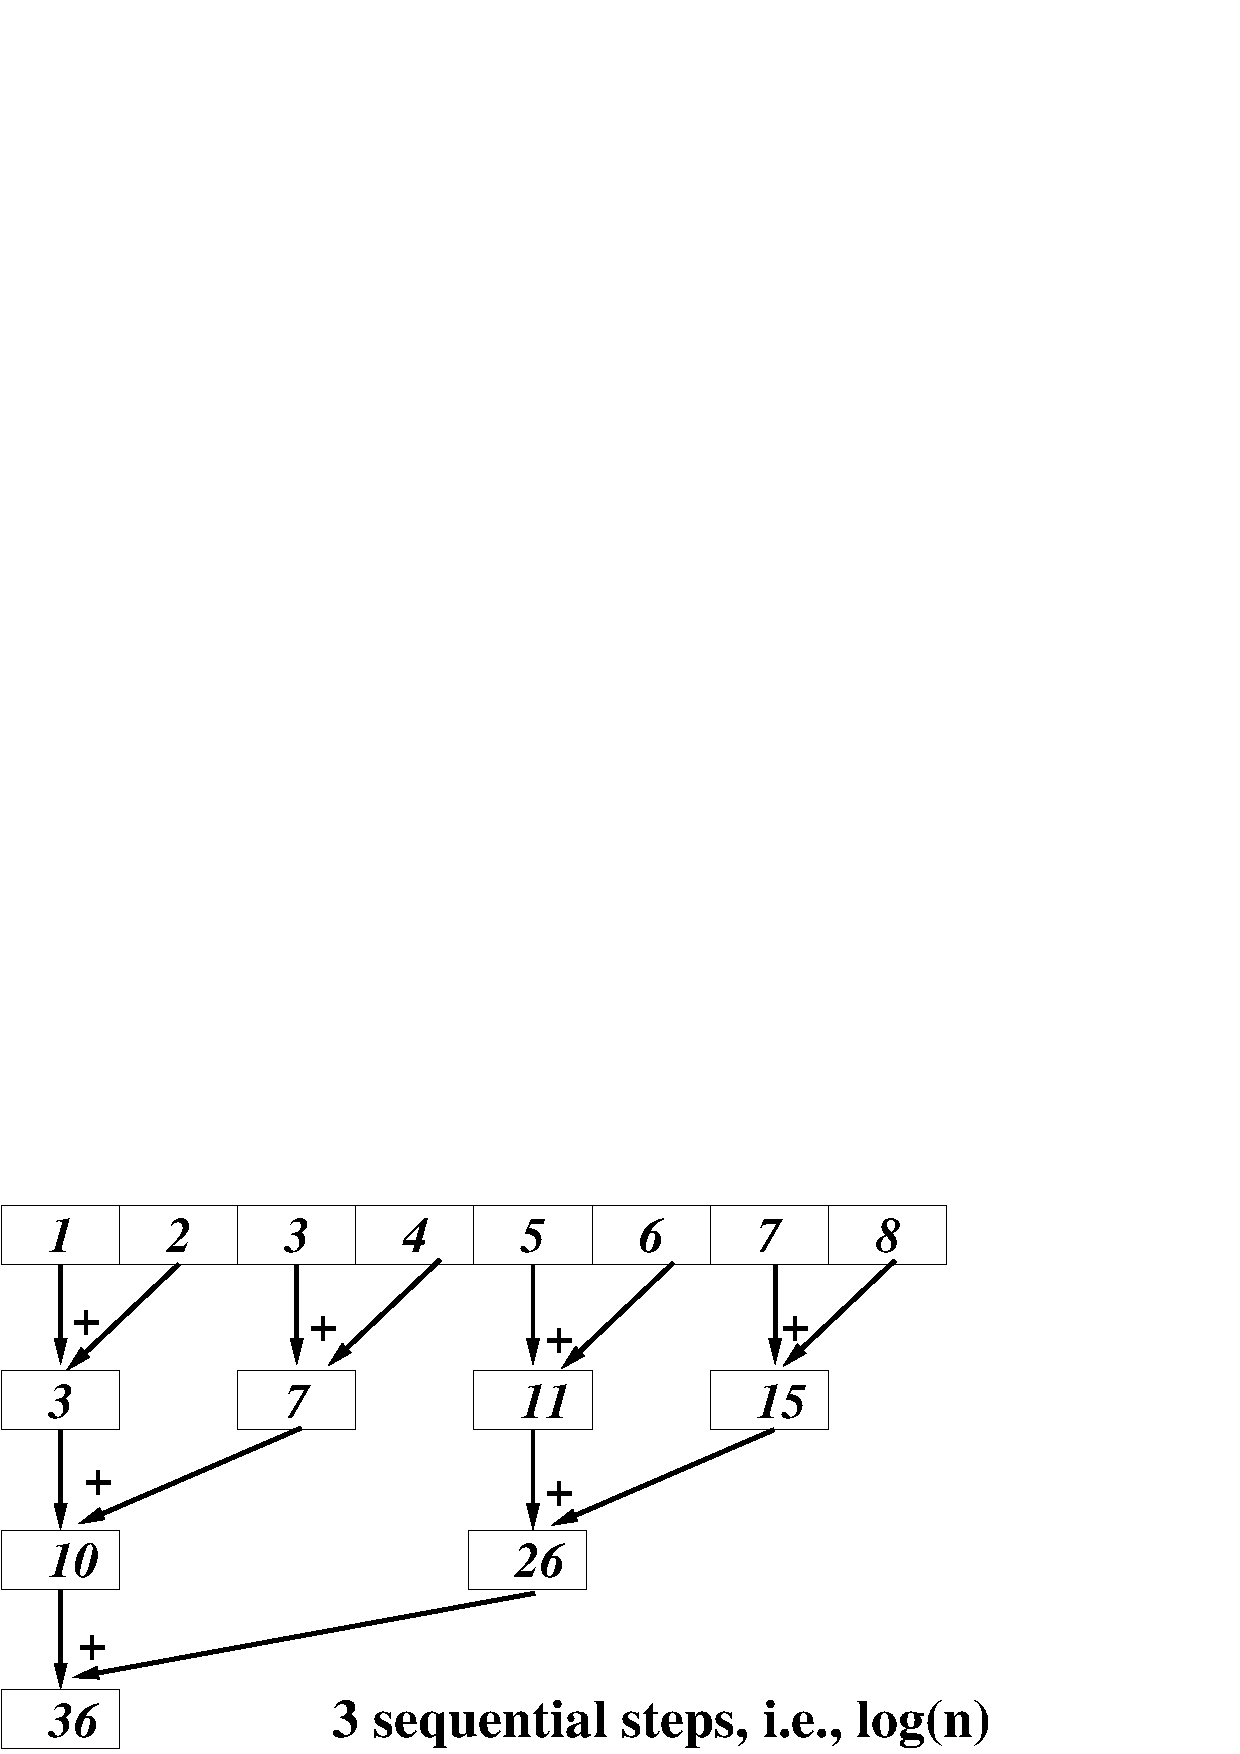
\includegraphics[height=18ex]{Figures/ReduceEg.pdf} 
\end{center} 

\end{frame}


\begin{frame}
  \begin{center}
    \Huge
    Futhark: a purely-functional data-parallel language\\\bigskip

    Compiler and benchmark publicly available at\\\bigskip

    http://futhark-lang.org/
  \end{center}
\end{frame}


\begin{frame}
  \begin{center}
    \Huge
    First Case Study:\\Brute-Force\\Nearest Neighbor\\in Futhark\\
  \end{center}
\end{frame}


\begin{frame}[fragile,t]
   \frametitle{Futhark: Finding The Nearest Neighbor (1-NN)}

Compute distances with a \emph{\tt map}; find minimal distance and 
associated (neighbor) index with a \emph{\tt reduce}.
\medskip

\begin{lstlisting}
let nearestNeigbor (current_point: (f32,f32)) 
                   (points: [#n](f32,f32)) : (f32,i32)
  let (lat, lng) = current_point
  let distances  =        -- computes all distances
      map (\ point ->     -- to the current point
                let (lat_i, lng_i) = point
                in f32.sqrt( (lat-lat_i)*(lat-lat_i) + 
                             (lng-lng_i)*(lng-lng_i) )
          ) points

  in  reduce minValInd (f32.inf,0) (zip distances (iota n))

-- associative and commutative operator.
let minValInd (vi1: (f32,i32)) (vi2: (f32,i32)) : (f32,i32) =
        let ((v1,i1), (v2,i2)) = (vi1, vi2)
        in  if      v1 < v2 then (v1, i1)
            else if v2 < v1 then (v2, i2)
            else if i1 < i2 then (v1, i1)
            else                 (v2, i2)
\end{lstlisting}

\end{frame}


\begin{frame}[fragile,t]
   \frametitle{Futhark: Finding k Nearest Neighbors (k-NN)}

The {\tt result} is now an array of size {\tt k}.\\
Each of the {\tt k} NNs is computed in a loop iteration, then the 
entry in {\tt distances} corresponding to the computed NN is set to 
$\infty$ so it will not be found again in following iterations. 
\medskip

\begin{lstlisting}
let nearestNeigbor (k: i32) (current_point: (f32,f32)) 
                   (points: [#n](f32,f32)) : [k](f32,i32)
  let (lat, lng) = current_point
  let distances = map ... -- as before

  let result = replicate k  (0i32, 0.0f32) -- init result
  loop ((result, distances)) = for i < k do
      let (minDist, minIndex) =
        reduce minValInd (f32.inf,0) (zip distances (iota n))

      let distances[minIndex] = f32.inf
      let result[i] = (minDist,minIndex)
      in (result, distances)
  in result
\end{lstlisting}

\end{frame}

\begin{frame}[fragile]
  \frametitle{Interoperability: Easy to Use from Python}

  \begin{enumerate}
  \item Create Futhark program \texttt{sum.fut}:
    \begin{lstlisting}
      entry int sum(int n) = reduce(+) 0 (iota n)
    \end{lstlisting}
  \item Compile it:\\
\begin{tinycode}
$ futhark-pyopencl --library sum.fut
\end{tinycode}
  \item Use the generated \texttt{sum.py} module from Python:
\begin{tinycode}
$ python
Python 2.7.11+ (default, Apr 17 2016, 14:00:29)
[GCC 5.3.1 20160409] on linux2
Type "help", "copyright", "credits" or "license" for more information.
>>> import sum
>>> s = sum.sum(interactive=True)
>>> s.sum(1000000)
1783293664
>>> 
\end{tinycode}
  \end{enumerate}

  \begin{itemize}
  \item The need to instantiate a class is to encapsulate OpenCL state and the like.
  \item This examples uses only scalars - arrays are passed and returned as Numpy arrays.
  \end{itemize}

\end{frame}


\begin{frame}
  \frametitle{Futhark Performance}

  Futhark compared to hand-written OpenCL and Accelerate (higher is
  better).

  \begin{center}
    \includegraphics[width=12cm]{img/speedup.pdf}
  \end{center}

\end{frame}


\begin{frame}
  \begin{center}
    \Huge
    Having Fun With Futhark:\\
    Visualization demonstrating\\
    Python Interoperability.

  \end{center}
\end{frame}

%%%%%%%%%%%%%%%%%%%%%%%%%%%
%%%%%%%% k-means %%%%%%%%%%
%%%%%%%%%%%%%%%%%%%%%%%%%%%

\begin{frame}
  \begin{center}
    \Huge
    Second Case Study:\\$k$-means Clustering\\in Futhark
  \end{center}
\end{frame}

\begin{frame}
  \frametitle{The Problem}

  We are given $n$ points in some $d$-dimensional space, which we must
  partition into $k$ disjoint sets, such that we minimise the
  inter-cluster sum of squares (the distance from every point in a
  cluster to the centre of the cluster).

  Example with $d=2, k=3, n=\textit{more than I can count}$:

  \begin{center}
    \includegraphics[width=50ex]{img/kmeans.png}
  \end{center}
\end{frame}

\begin{frame}
  \frametitle{The Solution (from Wikipedia)}
  \footnotesize
  \begin{tabular}{p{5cm}p{5cm}}
    \includegraphics[width=3cm]{img/kmeans1.png} & \includegraphics[width=3cm]{img/kmeans2.png} \\

    (1) $k$ initial "means" (here $k=3$) are randomly generated within the data domain. &

    (2) $k$ clusters are created by associating every observation with the nearest mean.\\

    \includegraphics[width=3cm]{img/kmeans3.png} & \includegraphics[width=3cm]{img/kmeans4.png} \\

    (3) The centroid of each of the $k$ clusters becomes the new mean. &

    (4) Steps (2) and (3) are repeated until convergence has been reached.
  \end{tabular}
\end{frame}

\begin{frame}[fragile,t]
  \frametitle{Step (1) in Futhark}

  \begin{tabular}{p{3cm}p{7cm}}
    \adjustimage{width=2cm,valign=m}{img/kmeans1.png} &
    $k$ initial "means"
    (here $k=3$) are randomly generated within the data domain.
  \end{tabular}
  \vspace{2em}

  \texttt{points} is the array of points - it is of type
  \texttt{ [n][d]f32}, i.e., an \texttt{n}~by~\texttt{d} array of
  32-bit floating point values.\medskip

  We assign the first \texttt{k} points as the initial (``random'')
  cluster centres:\medskip


  \begin{lstlisting}
let cluster_centres = map (\(i: int): [d]f32 -> points[i])
                          (iota k)
\end{lstlisting}

\end{frame}

\begin{frame}[fragile,t]
  \frametitle{Step (2) in Futhark}

  \begin{tabular}{p{2cm}p{7cm}}
    \adjustimage{width=2cm,valign=m}{img/kmeans2.png} &
    $k$ clusters are created by associating every observation with the nearest mean.
  \end{tabular}
  \vspace{2em}
  \begin{lstlisting}
-- Of type [int,n]
let new_membership =
   map (find_nearest_point cluster_centres) points
\end{lstlisting}

Where

\begin{lstlisting}
let find_nearest_point (cluster_centres: [k][d]f32)
                       (pt : [d]f32) : int =
  let (i,_) = reduce closest_point
                (0, euclid_dist_2 pt (cluster_centres[0]))
                (zip (iota npoints)
                     (map (euclid_dist_2 pt) cluster_centres))
  in i
\end{lstlisting}

\end{frame}

\begin{frame}[fragile,t]
  \frametitle{Step (3) in Futhark}

  \begin{tabular}{p{2cm}p{7cm}}
    \adjustimage{width=2cm,valign=m}{img/kmeans3.png} &
    The centroid of each of the $k$ clusters becomes the new mean.
  \end{tabular}

  \vspace{2em}

  \alert{This is the hard one.}

  \begin{lstlisting}
let new_centres =
  centroids_of k points new_membership
\end{lstlisting}

Where

\begin{lstlisting}
let centroids_of (k: int) (points: [n][d]f32)
                 (membership : [n]int) : [k][d]f32 =
  -- the number of points per cluster
  let cluster_sizes : [k]int = ...
  -- the cluster centres
  let cluster_centres : [k][d]f32 = ...
  in cluster_centres
\end{lstlisting}

\end{frame}

\begin{frame}[fragile]
  \frametitle{Computing Cluster Sizes: the Ugly}

  A sequential loop:

  \begin{lstlisting}
loop (counts = replicate(k,0)) =
  for i < n do
    let cluster = membership[i]
    let counts[cluster] = counts[cluster] + 1
    in counts
\end{lstlisting}

Loops are inherently sequential in Futhark:\\
this version is efficient only on sequential hardware.

\bigskip

Work efficient: $O(n)$

\end{frame}

\begin{frame}[fragile]
  \frametitle{Computing Cluster Sizes: the Bad}

  Use a parallel \texttt{map} to compute ``increments'', and then a
  \texttt{reduce} of these increments.

  \begin{lstlisting}
let increments =
  map (\(cluster: int) : [k]int ->
        let incr = replicate k 0
        let incr[cluster] = 1
        in  incr )
      membership

reduce(\(x: [k]int) (y: [k]int) : [k]int ->
         map (+) x y
      ) 
      (replicate k 0) increments
\end{lstlisting}

This is parallel, but not work-efficient $O(n\times k)$.
\end{frame}

\begin{frame}
  \frametitle{One Futhark Design Principle}

  \begin{block}{}
    The hardware is not infinitely parallel - ideally, we use an
    efficient sequential algorithm for chunks of the input, then use a
    parallel operation to combine the results of the sequential parts.
  \end{block}

%  \begin{center}
%    \includegraphics[width=7cm]{chunking.pdf}
%  \end{center}

  The optimal number of threads varies from case to case, so this
  should be abstracted from the programmer.
\end{frame}

\begin{frame}[fragile]
  \frametitle{Computing cluster sizes: the Good}

  We use a Futhark language construct called a \textit{reduction
    stream}.

  \begin{lstlisting}
  let cluster_sizes =
     streamRed(\(x: [k]int) (y: [k]int) : [k]int ->
                 map (+) x y
              )
              (\(acc:[k]int) (chunk:[@chunksize@]int): [k]int ->
                 loop (acc) = for i < @chunksize@ do
                   let cluster = chunk[i]
                   let acc[cluster] = acc[cluster] + 1
                   in acc
                 in acc
              )
              (replicate k 0) membership
\end{lstlisting}

We specify a sequential fold function and a parallel reduction
function.  The compiler is able to exploit as much parallelism as is
optimal on the hardware, and can use our sequential code inside each
thread.

\end{frame}

\begin{frame}[fragile]
  \frametitle{Back To Step (3)}

  Computing the actual cluster sums, now that we have
  \texttt{cluster\_sizes}, is straightforwardly done with another
  stream:

  \begin{lstlisting}
let cluster_sums = 
  streamRed
    (map (map (+))) -- matrix addition
    (\(acc:[k][d]f32) (chunk:[chksz]([d]f32,int)): [k][d]f32->
      loop (acc) = for i < chksz do
        let (point, cluster) = chunk[i]
        let acc[cluster] =
          map (+) acc[cluster]
                  (map (/cluster_sizes[cluster]) point)
        in acc
      in acc
    )
    (replicate k (replicate d 0.0))
    (zip points membership)
\end{lstlisting}
\end{frame}

\begin{frame}[fragile,t]
  \frametitle{Step (4) in Futhark}

  \begin{tabular}{p{2cm}p{7cm}}
    \adjustimage{width=2cm,valign=m}{img/kmeans4.png} &
    Steps (2) and (3) are repeated until convergence has been reached.
  \end{tabular}

  We iterate until we reach convergence (no points change cluster
  membership), or until we reach 500 iterations.  This is done with a
  \texttt{while}-loop:

  \begin{lstlisting}
loop ((membership, cluster_centres, delta, i)) =
  while delta > 0 && i < 500 do
    let new_membership =
      map (find_nearest_point cluster_centres) points
    let new_centres =
      centroids_of k points new_membership
    let delta =
      reduce (+) 0
             (map (\ (b: bool) : int ->
                      if b then 0 else 1
                  ) 
                  (map (==) membership new_membership))
    in (new_membership, new_centres, delta, i+1)
\end{lstlisting}

\end{frame}



\end{document}
